\documentclass[pdf, hyperref={unicode}, aspectratio=169]{beamer}

\usepackage{./styles11}

% Выключаю кнопочки
\setbeamertemplate{navigation symbols}{}

% Название темы слишком длинное, поменьше шрифт!
\setbeamerfont{title}{series=\bfseries, size=\large}

\useoutertheme{miniframes}

\graphicspath{ {/img/} }

\title{Горизонтальное масштабирование PostgreSQL для улучшения производительности при работе с крупными таблицами в условиях заданной схемы базы данных}

\subtitle{Выпускная квалификационная работа бакалавра}

% \pdfstringdefDisableCommands{
%   \def\\{}
%   \def\,{}
%   \def\textbf#1{<#1>}
% }

\author[Куценко Борис Дмитриевич]
{
  \textbf{Студент группы М8О-407Б-20:} Куценко Борис Дмитриевич\\
  \ \textbf{Научный руководитель:} ст. преподаватель кафедры 806\\\ Миронов Евгений Сергеевич
  % Обратите внимание на пробел в начале строки
}

\institute[Московский авиационный институт]
{
  Московский авиационный институт (национальный исследовательский университет)\\
  Институт № 8 «Компьютерные науки и прикладная математика»\\
  Кафедра № 806 «Вычислительная математика и программирование» 
}

\date{Москва --- \the\year}

\logo{
\includegraphics[height=1cm]{img/mai.eps}}

\begin{document}

\epstopdfsetup{outdir=./}

\setbeamertemplate{footline}{}
{
	% убирает номер слайда с титульного слайда
	\setbeamertemplate{page number in head/foot}{}
	\frame{\titlepage}
}




\section{Цель работы}
\begin{frame}
	\frametitle{Цель работы}
	
	\textbf{Цель} - разработать набор утилит и библиотеку для высокоуровневого языка программирования по управлению шардированием в PostgreSQL для бэкенд разработчиков
\end{frame}

\section{Актуальность темы}
\begin{frame}
	\frametitle{Актуальность темы}
	
	
	\begin{itemize}
		\item PostgreSQL - одна из ведущих реляционных СУБД с открытым исходным кодом
		\item Современные информационные системы сталкиваются с постоянным ростом объемов данных,
		что может привести  к исчерпанию ресурсов сервера и снижением производительности из-за ограничений по доступному месту и замедлении скорости обработки запросов.
		\item Горизонтальное масштабирование решает эти проблемы, но при использовании стандартных методов PostgreSQL, приходится перестраивать все существующие связи и схемы БД,
		что может привести к большим временным затратам
	\end{itemize}
\end{frame}


\begin{frame}
	\frametitle{Задачи работы}
	
	\textbf{Задачи:}
	\begin{enumerate}
		\fontsize{10pt}{12pt}\selectfont
		\item Выбрать и реализовать алгоритм для записи и чтения распределенных данных
		\item Спроектировать и реализовать библиотеку для высокоуровневого языка программирования по работе с распределенными данными, совместимую с существующими решениями по работе с БД
		\item Придумать решение проблемы неравномерного распределения данных при добавлении новых серверов, обеспечив балансировку нагрузки и равномерное хранение данных на шардах
		\item Реализовать механизм копирования данных с одного сервера на другой при изменении количества серверов
		\item Произвести тест производительности разработанного решения

	\end{enumerate}
\end{frame}

\section{Постановка задачи}
\begin{frame}
	\frametitle{Постановка задачи}
	
	При увеличении размера таблицы в базе данных возникают следующие проблемы
	
	\begin{itemize}
		\item Опереации чтения и записи замедляются
		\item Существует вероятность достижения максимального порога размера базы данных на сервере
	\end{itemize}
	Одним из способов решения данных проблем является горизонтальное масштабирование. PostgreSQL не предоставляет готового механизма для его организации в существующей схеме БД. Требуется создать набор утилит и библиотеку, которые бы обеспечили масштабирование базы данных при минимальном изменении существующей кодовой базы.
\end{frame}


\section{Стек технологий}
\begin{frame}
	\frametitle{Стек технологий}
	
	\begin{itemize}
		\item \textbf{Python} является основным языком программирования, который использовался при решении задачи;
		\item \textbf{PostgreSQL} СУБД для которого написано решение;
		\item \textbf{Docker} позволяет разворачивать и переносить изолированные контейнеры с базами данных;
	\end{itemize}
\end{frame}

\section{Архитектура решения, алгоритм решения задачи}
\begin{frame}
	\frametitle{Архитектура решения, алгоритм решения задачи}

	Существует два подхода к горизонтальному масштабированию
	\begin{enumerate}
		\item "на холодную" (Cold Scaling) - добавление или удаление ресурсов, требующее перезагрузки системы или её компонентов.
		\item "на горячую" (Live/Hot Scaling) - добавление или удаление ресурсов в реальном времени без остановки системы.
	\end{enumerate}
	Преимущества второго подхода
	\begin{itemize}
		\item Непрерывность работы: Система продолжает работать без прерываний.
		\item Минимизация простоев: Пользователи не замечают изменений.
	\end{itemize}
	
\end{frame}


\begin{frame}
	\frametitle{Архитектура решения, алгоритм решения задачи}
	% \centering
	\begin{minipage}{.6\textwidth}
			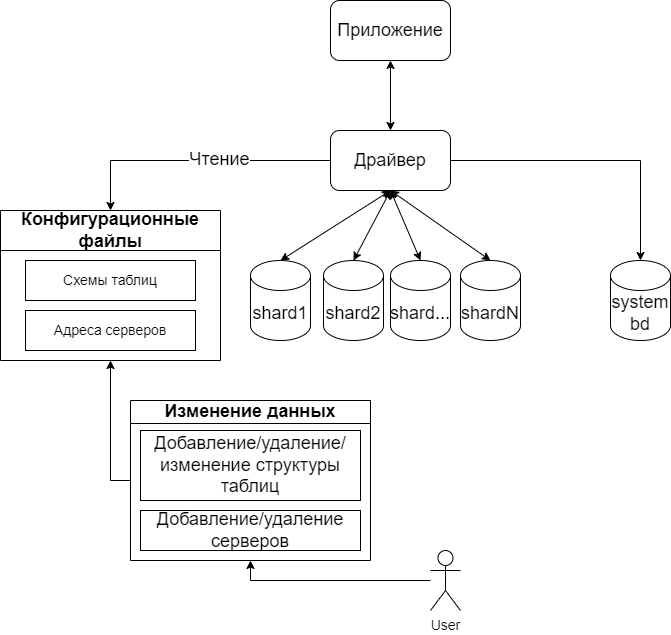
\includegraphics[width=\textwidth]{img/arch2.png}
	\end{minipage}%
	\begin{minipage}{.5\textwidth}
			\captionof{figure}{Архитектура решения}\label{fig:arch2}
	\end{minipage}
\end{frame}

\begin{frame}
	\frametitle{Архитектура решения, алгоритм решения задачи}
	Пример запроса

	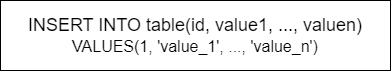
\includegraphics[height=9mm]{img/qeury1.png}

	Построение абстрактного синтаксическое дерева
	
	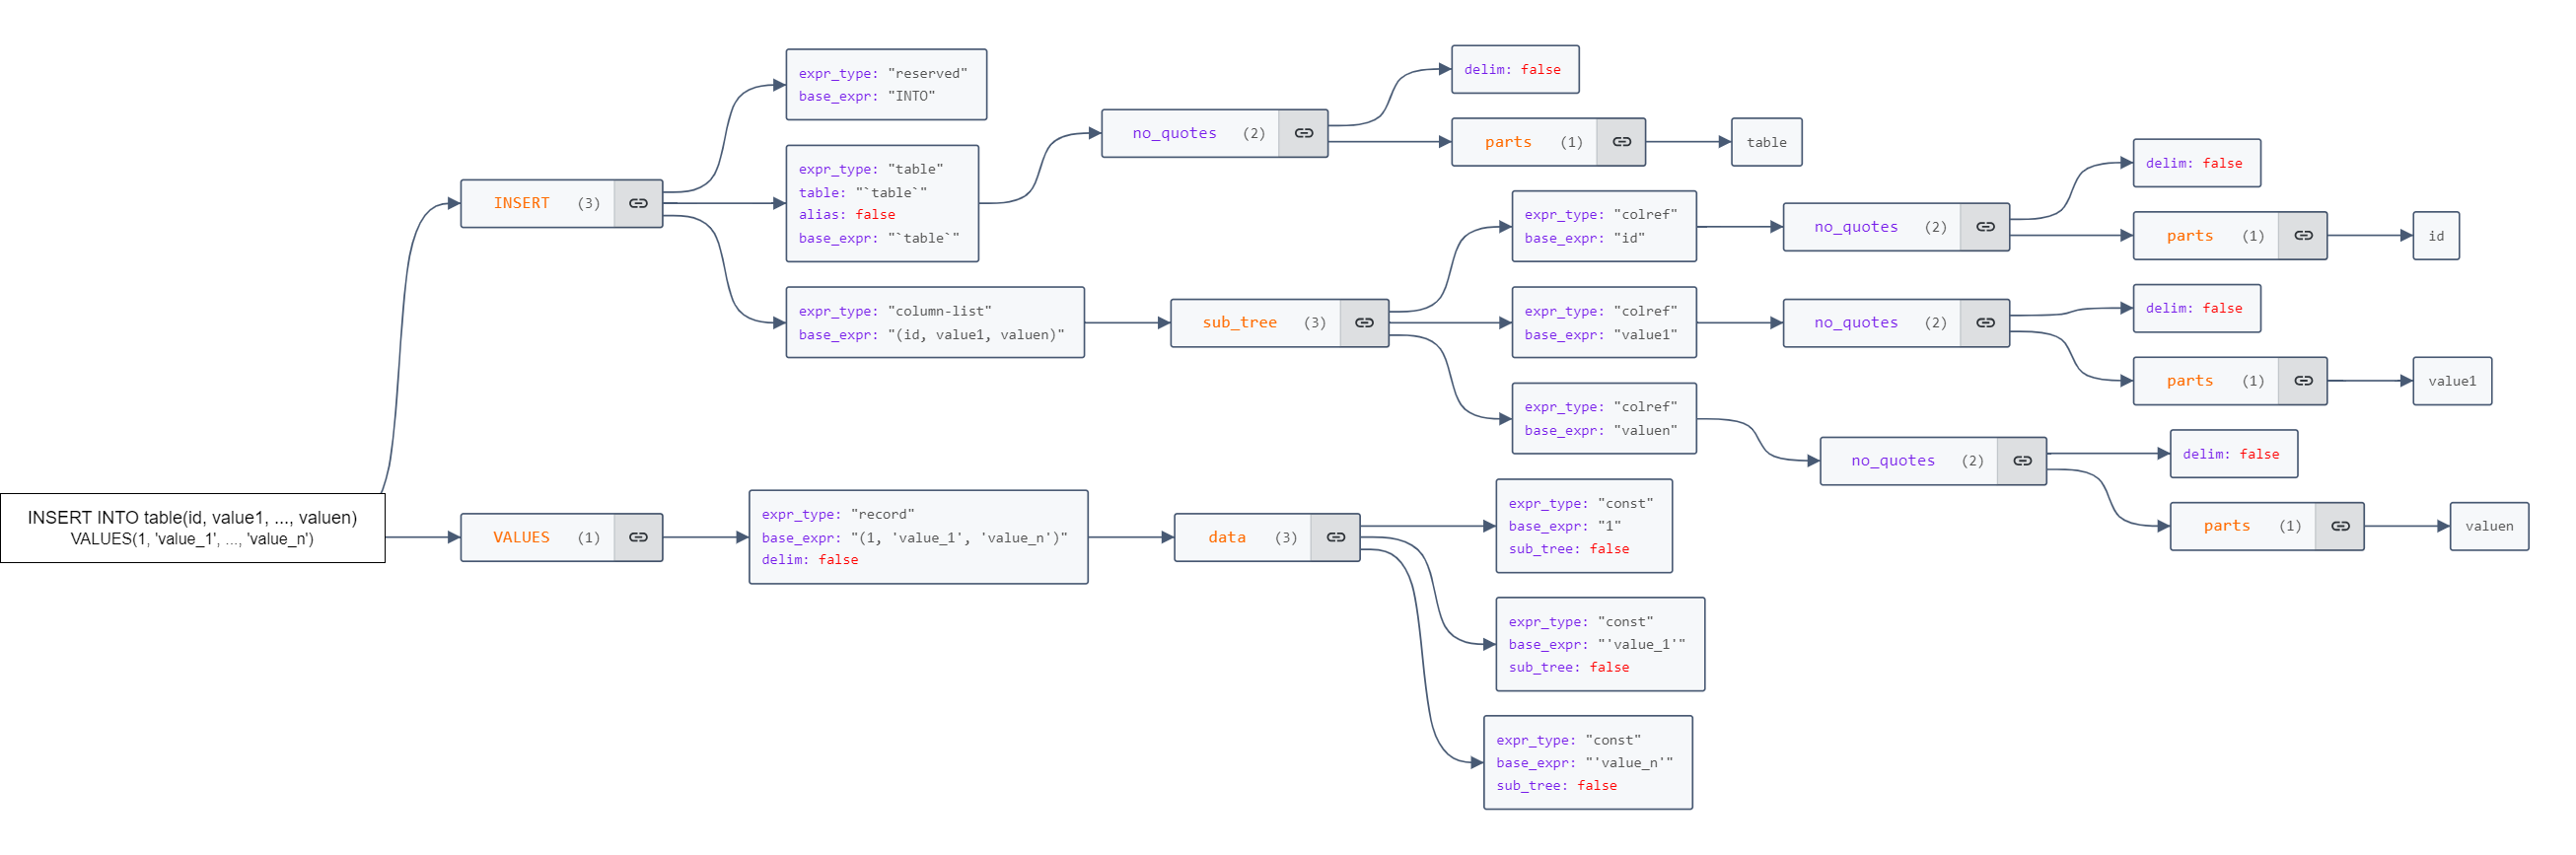
\includegraphics[width=\textwidth]{img/AST.png}

\end{frame}


\begin{frame}
	\frametitle{Архитектура решения, алгоритм решения задачи}
	\begin{minipage}{.6\textwidth}
		Генерация запросов из abstract syntax tree (AST)
		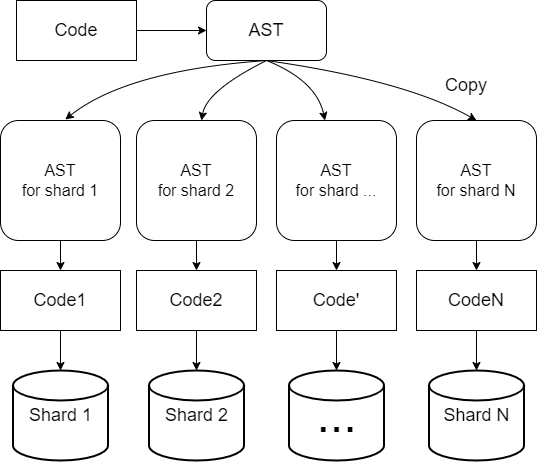
\includegraphics[width=\textheight]{img/generation.png}
	\end{minipage}%
	\begin{minipage}{.4\textwidth}
		Для каждого сервера создается новый SQL запрос, в котором присутствуют только те данные, которые относятся к данному
	\end{minipage}%
\end{frame}


\begin{frame}
	\frametitle{Архитектура решения, алгоритм решения задачи}
  
	\textbf{Как понять в какой сервер записывать данные?}
  
	\vspace{1.5em}
  
	Эту проблему решают следующие алгоритмы:
  
	\begin{enumerate}
		\item Хэширование по модулю
		\item Шардирование по последним битам ключа
		\item Шардирование с использованием битового бора (Trie-based шардирование)
		\item Шардирование с фиксированным числом "бакетов"
		\item Консистентное хэширование
		\item Рандеву-хэширование
	\end{enumerate}
\end{frame}

\begin{frame}
	\frametitle{Архитектура решения, алгоритм решения задачи}
	\textbf{Перебалансировка}

	\vspace{1.5em}
	\centering
	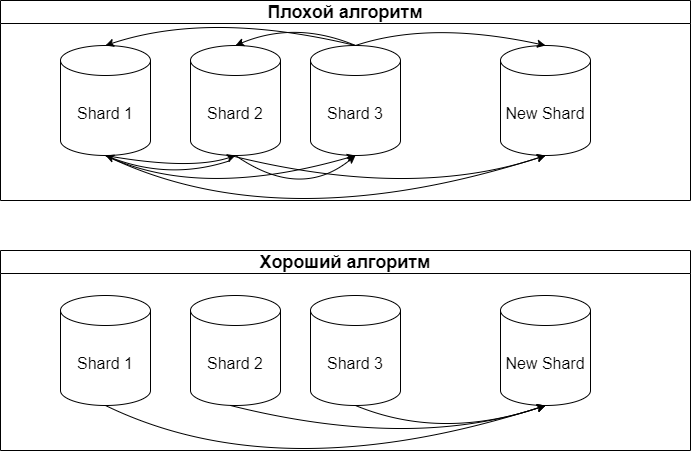
\includegraphics[width=\textheight]{img/resharding.png}


\end{frame}

\begin{frame}
	\frametitle{Архитектура решения, алгоритм решения задачи}
	\textbf{Перебалансировка}
	
	\vspace{1.5em}
	\centering
	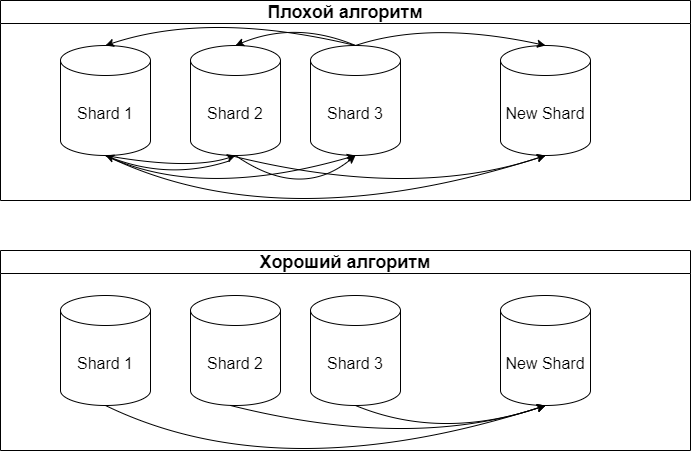
\includegraphics[width=\textheight]{img/resharding.png}
\end{frame}

\section{Список литературы}
\begin{frame}
	\frametitle{Список литературы}

	\begin{itemize}
		\item Консистентное хэширование:
		\begin{itemize}
			\item Karger, D.; Lehman, E.; Leighton, T.; Panigrahy, R.; Levine, M.; Lewin, D. (1997). Consistent Hashing and Random Trees: Distributed Caching Protocols for Relieving Hot Spots on the World Wide Web
			\item Roughgarden, Tim; Valiant, Gregory (28 March 2021). "The Modern Algorithmic Toolbox, Introduction to Consistent Hashing".
		\end{itemize} 

		\item Рандеву хэширование:
		\begin{itemize}
			\item Thaler, David; Chinya Ravishankar. "A Name-Based Mapping Scheme for Rendezvous"
		\end{itemize} 
		\item Документация PostgreSQL:
		\begin{itemize}
			\item https://www.postgresql.org/docs/current/index.html
		\end{itemize}
	\end{itemize}
\end{frame}


\end{document}